\documentclass{beamer}
\usepackage[german]{babel}

%\usepackage[activate={true,nocompatibility},final,tracking=true,kerning=true,spacing=true,factor=1100,stretch=10,shrink=10]{microtype}
\usepackage{paratype}
%\usepackage{libertine}
%\usepackage[scaled]{berasans}
\renewcommand*\familydefault{\sfdefault}  %%
\usepackage[utf8]{inputenc}

\usepackage[T1]{fontenc}


\usepackage{microtype}
\usepackage{xcolor}
\usepackage{pgffor}
%\usetheme{beamertheme-bjeldbak/beamerthemebjeldbak}
\usepackage{tikz}

\usepackage[absolute,overlay]{textpos}
%\usepackage[texcoord,grid,gridunit=mm,gridcolor=red!10,subgridcolor=green!10]{eso-pic}
\setbeamertemplate{navigation symbols}{}

\newcommand{\makemycolor}[2]{%
    \pgfmathsetmacro{\hue}{(#1/100)^1.715*0.79}%
    \definecolor{myhsbcolor}{hsb}{\hue,1,1}%
    \textcolor{myhsbcolor}{#2}%
}

\title{Lumineszenz von Seltenerd-Ionen}
\author{Nevroz Arslan}

\begin{document}
  {%
    \setbeamertemplate{headline}{}
    \frame{\titlepage}
  }

  \begin{frame}
\frametitle{There Is No Largest Prime Number}
\framesubtitle{The proof uses \textit{reductio ad absurdum}.}
    %\foreach \x in {300,320,...,900} {\textcolor[wave]{\x}{\x}\ }\\
    \begin{columns}
      \column{.5\textwidth}
               
       \begin{figure}[!htbp]
          \centering
          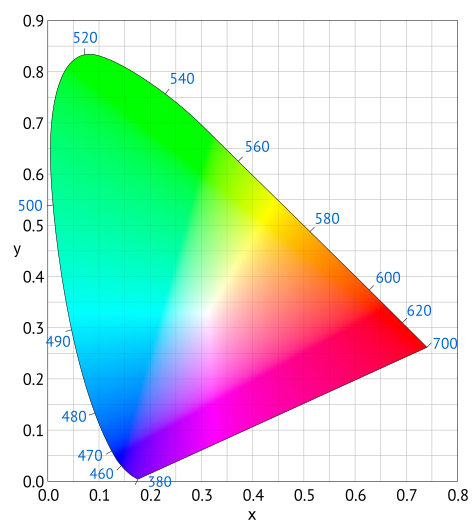
\includegraphics[width=\textwidth]{farbindex.png}
        \end{figure}
       
       \column{.5\textwidth}
            \begin{block}{Answered Questions}
          How many primes are there?
          \end{block}
      \end{columns}

  \end{frame}
  
\begin{frame}[t]\frametitle{ Seltenerdionen mit f$\rightarrow$d-Übergängen}
 \begin{beamerboxesrounded}[lower=block body,shadow=false]{f-d}
   \textbf{ Ein guter Leuchtstoff soll die Anregungsenergie möglichst effizient absorbieren und in Form von Licht wieder
   emittieren; das bedeutet, dass die Quantenausbeute [5] mög-
   lichst hoch sein soll.}
    \end{beamerboxesrounded}   

\end{frame}

  \begin{frame}[t]\frametitle{Farbtemperatur}

  \begin{tikzpicture}
    \foreach \k in {0,1,...,100}{%
        \pgfmathsetmacro{\hue}{(\k/100)^1.715*0.79}
        \definecolor{mycolor}{rgb:hsb}{\hue,1,1}
        \node[color=mycolor] () at (\k/10,0) {$\bullet$};
    }%
    \foreach \f in {0,1,...,10}{%
        \pgfmathtruncatemacro{\num}{\f*10}
        \node () at (\f,-.5) {\num};
    }
    \foreach \g/\h in {0/Rot,2/Orange,4/Gelb,6/Grün,8/Blau,10/Purpur}{%
        \pgfmathtruncatemacro{\num}{\g*10}
        \node at (\g,-1) {\makemycolor{\num}{\h}};
    }%
    \end{tikzpicture}

  \end{frame}

  %Folie 4 Auswahlregeln
  \begin{frame}[t]\frametitle{Laporte Verbot}
      
  
  
  \end{frame}



%http://www.rsc.org/chemistryworld/News/2009/September/01090901.asp
\end{document}

